%==============================================================================
% Rapport final - Honeypot Intelligent - M1SPRO
% Auteurs : Mohammed Sellak & Rachid Oubenazha
%
% COMPILATION (recommandee : Overleaf, ou TeX Live complet) :
%   pdflatex rapport.tex   (lancer 2 fois pour la table des matieres)
% Polices pro : TeX Gyre Pagella (corps) + Helvetica (titres).
% Si une police/package manque en local, compilez sur Overleaf (tout y est).
%==============================================================================
\documentclass[11pt,a4paper]{article}

%--- Encodage & langue -------------------------------------------------------
\usepackage[utf8]{inputenc}
\usepackage[T1]{fontenc}
\usepackage[french]{babel}

%--- Polices professionnelles ------------------------------------------------
\usepackage{tgpagella}                 % corps : Palatino (elegant, lisible)
\usepackage[scaled=0.92]{helvet}       % titres : sans-serif type Helvetica
\usepackage{microtype}                 % justification fine, rendu pro

%--- Mise en page ------------------------------------------------------------
\usepackage[a4paper,margin=2.4cm,headheight=14pt]{geometry}
\usepackage{graphicx}
\usepackage{xcolor}
\usepackage{booktabs}
\usepackage{longtable}
\usepackage{array}
\usepackage{enumitem}
\usepackage{fancyhdr}
\usepackage{listings}
\usepackage{tikz}
\usetikzlibrary{positioning,arrows.meta,fit,backgrounds}
\usepackage{titlesec}
\usepackage{caption}
\usepackage[most]{tcolorbox}
\usepackage[hidelinks]{hyperref}
\hypersetup{colorlinks=true,linkcolor=primary,urlcolor=accent,citecolor=accent}

%--- Palette de couleurs professionnelle -------------------------------------
\definecolor{primary}{HTML}{12284C}   % bleu marine
\definecolor{accent}{HTML}{1F6FEB}    % bleu accent
\definecolor{ok}{HTML}{1A7F37}        % vert
\definecolor{warn}{HTML}{B7791F}      % ambre
\definecolor{danger}{HTML}{B91C1C}    % rouge
\definecolor{light}{HTML}{F2F5FA}     % fond clair
\definecolor{rulec}{HTML}{D0D7DE}     % filets
\definecolor{codebg}{HTML}{F6F8FA}
\definecolor{codekw}{HTML}{0550AE}
\definecolor{codestr}{HTML}{0A7B34}
\definecolor{codecmt}{HTML}{6E7781}

%--- En-tetes / pieds --------------------------------------------------------
\pagestyle{fancy}
\fancyhf{}
\lhead{\small\sffamily\color{primary}\textbf{Honeypot Intelligent}}
\rhead{\small\sffamily\color{primary}M1SPRO}
\lfoot{\small\sffamily\color{rulec!40!black}Sellak \& Oubenazha}
\rfoot{\small\sffamily\thepage}
\renewcommand{\headrulewidth}{0.6pt}
\renewcommand{\headrule}{\hbox to\headwidth{\color{accent}\leaders\hrule height \headrulewidth\hfill}}

%--- Titres de sections (sans-serif, marine, filet accent) -------------------
\titleformat{\section}{\sffamily\Large\bfseries\color{primary}}{\thesection.}{0.5em}{}[{\color{accent}\titlerule[1pt]}]
\titleformat{\subsection}{\sffamily\large\bfseries\color{accent!85!black}}{\thesubsection}{0.5em}{}
\titleformat{\subsubsection}{\sffamily\normalsize\bfseries\color{primary!85!black}}{\thesubsubsection}{0.5em}{}
\titlespacing*{\section}{0pt}{16pt}{8pt}

%--- Legendes ----------------------------------------------------------------
\captionsetup{font=small,labelfont={sf,bf,color=primary},labelsep=endash}

%--- Listings ----------------------------------------------------------------
\lstset{
  backgroundcolor=\color{codebg},
  frame=single, rulecolor=\color{rulec},
  basicstyle=\ttfamily\footnotesize,
  keywordstyle=\color{codekw}\bfseries,
  stringstyle=\color{codestr},
  commentstyle=\color{codecmt}\itshape,
  numbers=left, numberstyle=\tiny\color{codecmt}, numbersep=8pt,
  breaklines=true, showstringspaces=false, tabsize=2,
  captionpos=b, xleftmargin=16pt, framexleftmargin=16pt,
}

%--- Boites pro --------------------------------------------------------------
\newtcolorbox{resumebox}{enhanced,colback=light,colframe=accent,boxrule=0.8pt,
  arc=3pt,left=10pt,right=10pt,top=8pt,bottom=8pt,
  title=\sffamily\bfseries Resume executif,fonttitle=\color{white},coltitle=white,
  colbacktitle=accent,attach boxed title to top left={xshift=8pt,yshift=-2mm},
  boxed title style={colframe=accent,arc=2pt}}
\newtcolorbox{keybox}{enhanced,colback=ok!6,colframe=ok,boxrule=0.7pt,arc=3pt,
  left=10pt,right=10pt,top=6pt,bottom=6pt}
\newtcolorbox{warnbox}{enhanced,colback=warn!8,colframe=warn,boxrule=0.7pt,arc=3pt,
  left=10pt,right=10pt,top=6pt,bottom=6pt}

\newcommand{\chip}[2]{\textcolor{#1}{\textbf{#2}}}

%==============================================================================
\begin{document}

%--- PAGE DE GARDE -----------------------------------------------------------
\begin{titlepage}
\thispagestyle{empty}
\begin{tikzpicture}[remember picture,overlay]
  \fill[primary] (current page.north west) rectangle ([yshift=-4.6cm]current page.north east);
  \fill[accent]  ([yshift=-4.6cm]current page.north west) rectangle ([yshift=-4.9cm]current page.north east);
  \node[white,anchor=west,font=\sffamily\bfseries\Huge] at ([shift={(2.4cm,-2.4cm)}]current page.north west){Honeypot Intelligent};
  \node[white,anchor=west,font=\sffamily\large] at ([shift={(2.4cm,-3.4cm)}]current page.north west){Detection \& analyse comportementale des attaques};
\end{tikzpicture}

\vspace*{6.2cm}
\noindent\begin{tcolorbox}[enhanced,colback=light,colframe=rulec,boxrule=0.6pt,arc=3pt,left=14pt,right=14pt,top=10pt,bottom=10pt]
\sffamily\large\color{primary}\textbf{Rapport final de projet}\\[2pt]
\normalsize\color{black} Honeypot multi-services (SSH / HTTP / FTP), pipeline d'analyse en temps reel et generation de renseignement sur les menaces (CTI).
\end{tcolorbox}

\vfill
\noindent\renewcommand{\arraystretch}{1.35}
\begin{tabular}{@{}>{\sffamily\bfseries\color{primary}}l l@{}}
 Auteurs & Mohammed Sellak \\
         & Rachid Oubenazha \\
 Formation & Master 1 -- Securite des Systemes (M1SPRO) \\
 Etablissement & Ecole IT d'Amiens \\
 Module & Projet Honeypot -- 35 heures \\
 Date & \today \\
\end{tabular}
\vspace{1.4cm}
\end{titlepage}

%--- RESUME + SOMMAIRE -------------------------------------------------------
\begin{resumebox}
Ce projet realise un \textbf{honeypot intelligent multi-services} concu pour attirer,
capturer et analyser les attaques visant des services exposes. Au-dela de la simple
capture, le systeme constitue une \textbf{chaine complete de renseignement sur les
menaces} : chaque interaction est journalisee de maniere integre (signature
HMAC-SHA256), enrichie (geolocalisation, reputation), classee selon un profil
comportemental, visualisee en temps reel sur un tableau de bord de type SOC, puis
exportee vers des formats defensifs standards (Sigma, STIX~2.1, listes iptables).
\medskip

Lors de la campagne de validation, le systeme a capture \textbf{5\,899 evenements} sur
les trois services, avec \textbf{0 log corrompu} (integrite verifiee de bout en bout),
et a classe automatiquement les attaquants en quatre profils. L'audit de detectabilite
montre une progression de la furtivite de \textbf{6/30 a 21/30} apres durcissement.
\end{resumebox}

\medskip
{\sffamily\large\bfseries\color{primary}Sommaire}
\vspace{-0.4cm}
\renewcommand{\contentsname}{}
\tableofcontents
\newpage

%==============================================================================
\section{Introduction et contexte}
%==============================================================================
Tout service expose sur un reseau subit un bruit d'attaque permanent : balayages
automatises, attaques par force brute, tentatives d'exploitation de vulnerabilites.
Distinguer une activite reellement malveillante d'un balayage de routine est difficile,
et la collecte de renseignement exploitable reste un enjeu central pour toute equipe
defensive (Blue Team).

\subsection{Objectifs du projet}
Le projet poursuit deux objectifs complementaires :
\begin{enumerate}[leftmargin=1.5em,itemsep=2pt]
  \item \textbf{Detourner} une partie du trafic offensif vers des leurres sans valeur,
        afin d'observer les techniques adverses sans exposer de ressource reelle ;
  \item \textbf{Transformer} les interactions capturees en renseignement structure et
        directement exploitable (visualisation temps reel + exports CTI).
\end{enumerate}

\subsection{Perimetre et contraintes}
Le systeme couvre trois protocoles representatifs (SSH, HTTP, FTP), s'execute
entierement en conteneurs et doit rester \textbf{passif}, \textbf{securise} et
\textbf{conforme} au cadre legal (RGPD, article 323-1 du Code penal).

%==============================================================================
\section{Cadre theorique et choix de conception}
%==============================================================================
\subsection{Taxonomie de Spitzner}
Selon la taxonomie de L.~Spitzner, on distingue trois niveaux d'interaction. Le tableau
ci-dessous resume le compromis associe a chacun.

\begin{table}[h]\centering\small
\renewcommand{\arraystretch}{1.2}
\begin{tabular}{@{}lll@{}}
\toprule
\rowcolor{primary!8}\textbf{Niveau} & \textbf{Donnees recoltees} & \textbf{Risque} \\
\midrule
Faible & Connexions, bannieres & Tres faible \\
\textbf{Moyen (choisi)} & \textbf{Identifiants, commandes, payloads} & \textbf{Maitrise} \\
Fort & Comportement post-exploitation complet & Eleve (pivot) \\
\bottomrule
\end{tabular}
\caption{Compromis richesse / risque des niveaux d'interaction.}
\end{table}

\subsection{Justification du medium-interaction}
Nous retenons le niveau \textbf{moyen}. Il offre le meilleur ratio richesse/risque : un
faux shell et des reponses applicatives credibles donnent l'illusion d'un systeme reel
\emph{sans jamais exposer un systeme d'exploitation exploitable}. Cette approche
s'aligne sur le framework \textbf{MITRE Engage} (objectifs \textit{Collect},
\textit{Detect}, \textit{Direct}, \textit{Reassure}).

%==============================================================================
\section{Architecture du systeme}
%==============================================================================
L'architecture suit un flux unique, de l'attaquant jusqu'au renseignement defensif.
La figure~\ref{fig:archi} en presente la vue d'ensemble.

\begin{figure}[h]\centering
\begin{tikzpicture}[font=\sffamily\scriptsize,
  node distance=7mm and 9mm,
  base/.style={draw,rounded corners=2.5pt,minimum height=9mm,minimum width=20mm,inner xsep=5pt,align=center,line width=.6pt},
  atk/.style={base,fill=danger!10,draw=danger},
  svc/.style={base,fill=accent!12,draw=accent},
  proc/.style={base,fill=ok!10,draw=ok},
  store/.style={base,fill=warn!14,draw=warn},
  out/.style={base,fill=primary!12,draw=primary},
  arr/.style={-{Stealth[length=2.2mm]},line width=.7pt,draw=primary!75}]
  % Rangee A (gauche -> droite)
  \node[atk](atk){Attaquants\\ Hydra, Nikto};
  \node[svc,right=of atk](svc){3 services leurres\\ SSH / HTTP / FTP};
  \node[proc,right=of svc](logs){Logs JSON\\ signes HMAC};
  \node[proc,right=of logs](ship){Shipper};
  % Rangee B (sous ship, flux vers la gauche)
  \node[proc,below=10mm of ship](api){API\\ ingestion};
  \node[proc,left=of api](enr){Enrichissement\\ GeoIP + AbuseIPDB};
  \node[proc,left=of enr](cls){Classifier\\ 4 profils};
  \node[store,left=of cls](db){SQLite};
  \node[out,left=of db](dash){Dashboard\\ temps reel};
  \node[out,below=8mm of cls](exp){Exports\\ Sigma / STIX / iptables};
  % Fleches
  \draw[arr](atk)--(svc); \draw[arr](svc)--(logs); \draw[arr](logs)--(ship);
  \draw[arr](ship)--(api);
  \draw[arr](api)--(enr); \draw[arr](enr)--(cls); \draw[arr](cls)--(db); \draw[arr](db)--(dash);
  \draw[arr](cls)--(exp);
  % Cadre Docker
  \begin{scope}[on background layer]
    \node[draw=primary!40,dashed,rounded corners,fit=(svc)(logs)(ship)(api)(enr)(cls)(db)(dash)(exp),inner sep=5pt,label={[primary!70,font=\sffamily\tiny]north east:Docker Compose -- 6 conteneurs isoles}]{};
  \end{scope}
\end{tikzpicture}
\caption{Architecture de bout en bout : de l'attaque au renseignement defensif.}
\label{fig:archi}
\end{figure}

\subsection{Choix techniques}
\begin{table}[h]\centering\small
\renewcommand{\arraystretch}{1.2}
\begin{tabular}{@{}lll@{}}
\toprule
\rowcolor{primary!8}\textbf{Composant} & \textbf{Technologie} & \textbf{Justification} \\
\midrule
SSH & Python \texttt{asyncssh} & Controle total du handshake et du faux shell \\
HTTP & Python \texttt{FastAPI} & Routage simple, middleware d'en-tetes \\
FTP & Python \texttt{pyftpdlib} & Serveur FTP scriptable, hooks d'evenements \\
Ingestion & FastAPI + SQLite & Leger, sans serveur, suffisant au volume \\
Tableau de bord & Dash / Plotly & Visualisation temps reel en Python \\
Orchestration & Docker Compose & Reproductibilite, isolation reseau \\
Integrite & HMAC-SHA256 & Valeur probante des journaux (M1CRYP) \\
\bottomrule
\end{tabular}
\caption{Pile technique retenue et justifications.}
\end{table}

%==============================================================================
\section{Les services leurres}
%==============================================================================
\subsection{Service SSH (port 2222)}
Le service capture chaque couple identifiant/mot de passe. Les identifiants faibles sont
acceptes, ouvrant un \textbf{faux shell} (hostname \texttt{srv-prod-debian}) qui repond
de maniere coherente aux commandes courantes (\texttt{uname~-a}, \texttt{id},
\texttt{ps~aux}, \texttt{netstat}, \texttt{cat~/etc/passwd}, \texttt{history}...). La
banniere est alignee sur une Debian~12 reelle : \texttt{SSH-2.0-OpenSSH\_9.2p1
Debian-2+deb12u3}.

\subsection{Service HTTP (port 8080)}
Un serveur FastAPI expose des routes deliberement appatantes : \texttt{/.env},
\texttt{/.git/config}, \texttt{/phpinfo.php}, \texttt{/wp-login.php}, \texttt{/admin},
\texttt{/api/v1/users}. Un middleware reecrit les en-tetes pour simuler
\texttt{Apache/2.4.57 (Debian)} avec \texttt{X-Powered-By: PHP/8.1.2}, la pile Python
etant masquee (\texttt{server\_header=False}).

\subsection{Service FTP (port 2121)}
Le serveur annonce \texttt{220 (vsFTPd 3.0.5)} et propose un faux systeme de fichiers
appatant (\texttt{secrets.txt}, \texttt{db\_dump.sql}, \texttt{backup.zip}). Les actions
USER, PASS, LIST et RETR sont integralement journalisees.

\subsection{Integrite des preuves}
Chaque evenement est signe en \textbf{HMAC-SHA256}. L'ingestion recalcule la signature ;
toute alteration incremente le compteur \texttt{integrity\_failures}. Cette mesure
garantit la valeur probante des journaux, indispensable a un usage forensique.

%==============================================================================
\section{Pipeline d'analyse et classification}
%==============================================================================
\subsection{Contrat de log versionne}
Les composants communiquent via un schema JSON versionne (\texttt{schema\_version}
1.0.0), valide a l'ingestion (\texttt{additionalProperties:false}).

\begin{lstlisting}[language=,caption={Exemple d'evenement signe.}]
{
  "schema_version": "1.0.0",
  "event_id": "a1b2c3...",
  "timestamp": "2026-06-11T15:12:25Z",
  "service": "ssh",
  "src_ip": "172.18.0.1",
  "session_id": "e7f8...",
  "action": "login_attempt",
  "username": "root",
  "password": "123456",
  "integrity": "hmac-sha256:9f8a7b..."
}
\end{lstlisting}

\subsection{Enrichissement}
Chaque adresse IP source est enrichie par geolocalisation (base GeoLite2-City) et, si une
cle est fournie, par le score de reputation \textbf{AbuseIPDB}. Le mode degrade
(hors-ligne) est gere proprement : absence d'enrichissement plutot qu'echec du pipeline.

\subsection{Classification comportementale}
Le classifieur agrege les evenements par session et applique une heuristique
\textbf{explicable}, dont les seuils sont externalises dans \texttt{profiles.json}.

\begin{table}[h]\centering\small
\renewcommand{\arraystretch}{1.25}
\begin{tabular}{@{}p{3.1cm}p{6.4cm}p{3.2cm}@{}}
\toprule
\rowcolor{primary!8}\textbf{Profil} & \textbf{Heuristique principale} & \textbf{MITRE ATT\&CK} \\
\midrule
\chip{danger}{bruteforcer} & $\geq$ 8 tentatives d'authentification, cadence elevee & T1110 Brute Force \\
\chip{warn}{bot} & User-Agent automatise OU chemins / payloads d'exploit & T1595, T1190 \\
\textbf{human} & Commandes shell variees, rythme humain & T1059, T1083 \\
\chip{ok}{scanner\_legitimate} & UA Shodan/Censys/GreyNoise, faible volume & T1595 \\
\bottomrule
\end{tabular}
\caption{Les quatre profils comportementaux et leur correspondance ATT\&CK.}
\end{table}

Le classifieur retourne un objet \texttt{\{profil, confiance, raisons, mitre\}}, ce qui
rend chaque decision \textbf{auditable} : il ne s'agit pas d'une boite noire.

%==============================================================================
\section{Resultats et tableau de bord}
%==============================================================================
Le tableau de bord (figure~\ref{fig:dash}) restitue l'etat du systeme en temps reel
(rafraichissement toutes les 3~secondes) : indicateurs cles, services surveilles, carte
geographique, repartition des profils, volumetrie par service et identifiants les plus
testes.

\begin{figure}[h]\centering
\fbox{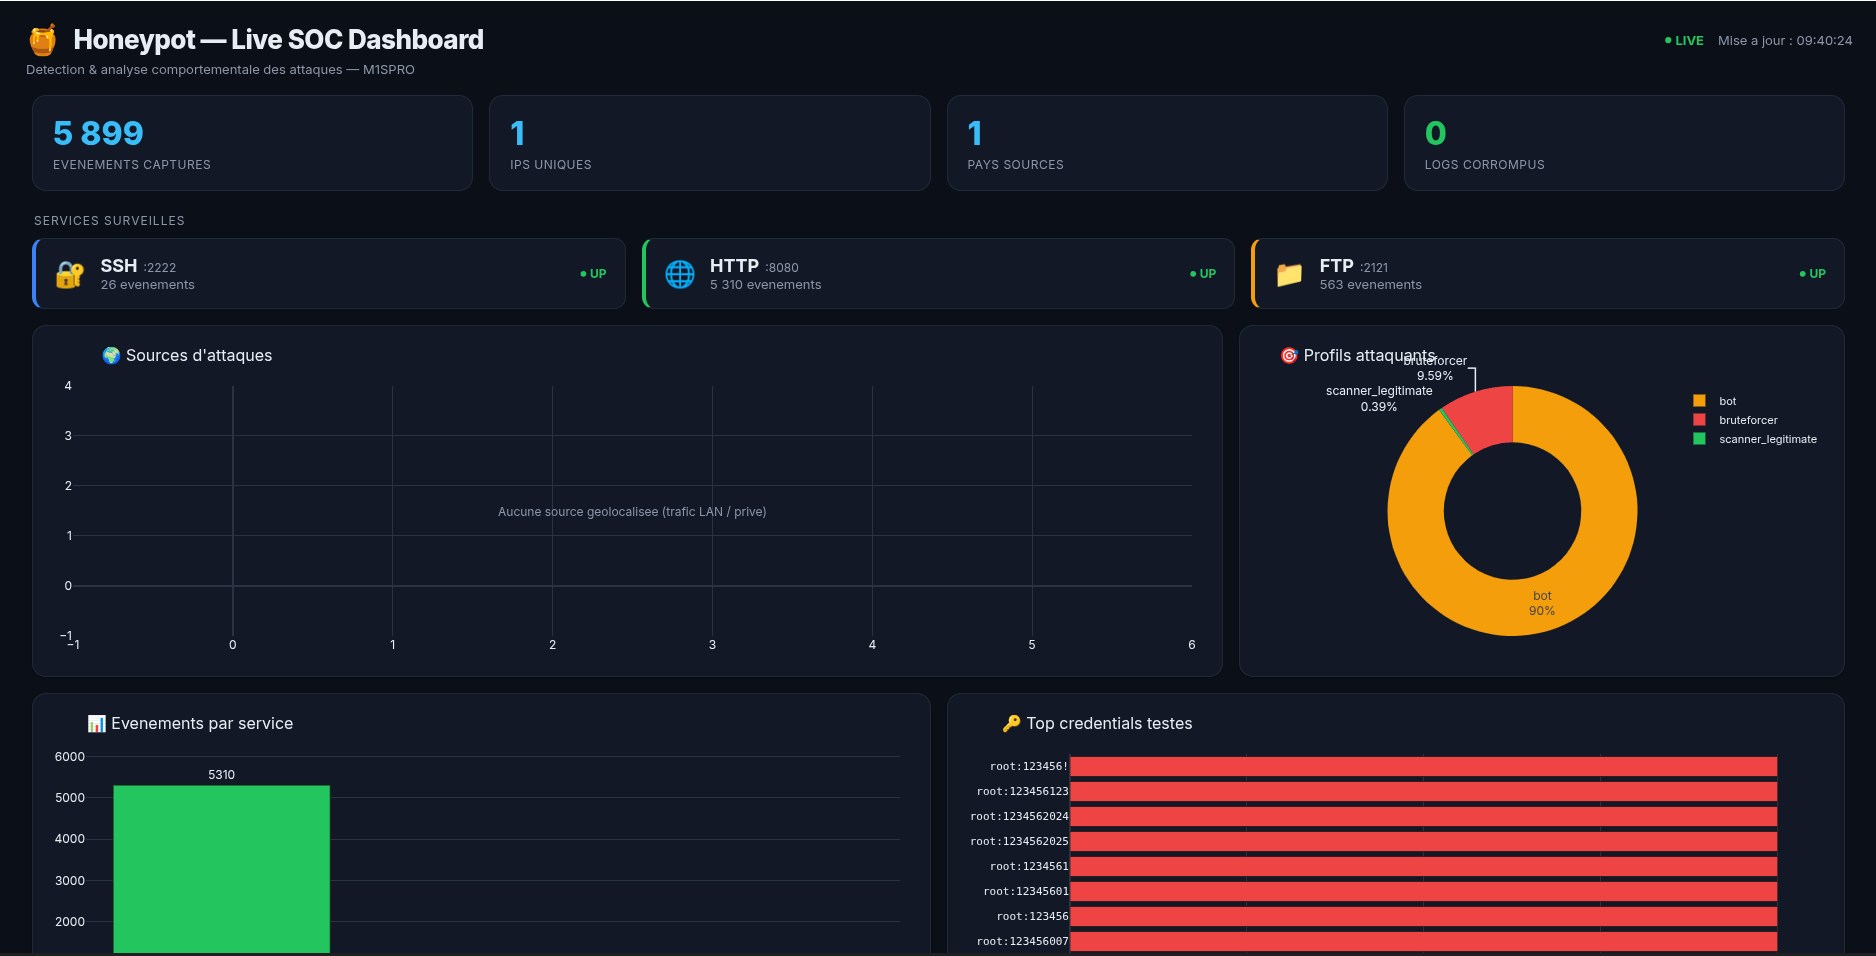
\includegraphics[width=\linewidth]{img/dashboard.png}}
\caption{Tableau de bord temps reel (\og Live SOC Dashboard \fg{}) durant la campagne de validation.}
\label{fig:dash}
\end{figure}

\subsection{Lecture des resultats}
La campagne a produit les chiffres suivants, directement lisibles sur le tableau de bord :

\begin{table}[h]\centering\small
\renewcommand{\arraystretch}{1.2}
\begin{tabular}{@{}lr@{\hspace{2.4em}}lr@{}}
\toprule
\rowcolor{primary!8}\textbf{Indicateur} & \textbf{Valeur} & \textbf{Service} & \textbf{Evenements} \\
\midrule
Evenements captures & 5\,899 & SSH (:2222) & 26 \\
IPs uniques & 1 & HTTP (:8080) & 5\,310 \\
Pays sources & 1 & FTP (:2121) & 563 \\
Logs corrompus & 0 & \textbf{Total} & \textbf{5\,899} \\
\bottomrule
\end{tabular}
\caption{Indicateurs globaux et volumetrie par service.}
\end{table}

\subsection{Interpretation}
\begin{itemize}[leftmargin=1.5em,itemsep=3pt]
  \item \textbf{Domination du HTTP (5\,310 evenements).} Le scan Nikto genere un tres
        grand nombre de requetes : c'est attendu et coherent avec un balayage de
        vulnerabilites. Ces sessions sont logiquement classees \chip{warn}{bot}
        (90~\% des profils).
  \item \textbf{Force brute SSH.} Les tentatives Hydra sur SSH alimentent le profil
        \chip{danger}{bruteforcer} (9,59~\%) ; les identifiants les plus testes sont des
        variantes de \texttt{root:123456}, typiques des dictionnaires d'attaque.
  \item \textbf{Scanners legitimes (0,39~\%).} Quelques sessions a faible volume avec un
        User-Agent connu sont correctement isolees, evitant les faux positifs.
  \item \textbf{Integrite parfaite (0 corrompu).} La verification HMAC valide la chaine
        de bout en bout : aucune preuve n'a ete alteree.
  \item \textbf{Carte vide \og trafic LAN/prive \fg{}.} En environnement de test, le
        trafic provient d'une machine attaquante locale : l'adresse n'est pas
        geolocalisable. En exposition reelle, la carte se remplirait avec les pays
        sources. Cette limite est \textbf{assumee} et documentee.
\end{itemize}

%==============================================================================
\section{Validation par attaques reelles}
%==============================================================================
Des scripts reproductibles rejouent des attaques representatives :
\begin{itemize}[leftmargin=1.5em,noitemsep]
  \item \textbf{Hydra} : force brute SSH et FTP (listes \texttt{rockyou-top1000}) ;
  \item \textbf{Nikto} et requetes ciblees : scan de vulnerabilites HTTP ;
  \item payloads d'exploitation (\texttt{/.env}, marqueurs Log4Shell).
\end{itemize}

Un script verifie automatiquement le bon fonctionnement de la chaine :

\begin{lstlisting}[language=,caption={Sortie de \texttt{attacks/assertions.py}.}]
[PASS] >= 50 evenements captures        (5899)
[PASS] service ssh present
[PASS] service http present
[PASS] profil bruteforcer detecte
[PASS] integrite des logs OK            (0 corrompu)
-> 5/5 assertions reussies
\end{lstlisting}

\begin{keybox}
\textbf{Resultat :} l'ensemble de la chaine (capture, transport, ingestion,
enrichissement, classification, persistance, restitution) est valide par 5 assertions
sur 5, sur un volume reel de pres de 6\,000 evenements.
\end{keybox}

%==============================================================================
\section{Audit de detectabilite (furtivite)}
%==============================================================================
Un honeypot n'a de valeur que s'il n'est pas trivialement identifie comme tel. Nous avons
mene un \textbf{audit avant/apres} avec les memes outils : \texttt{nmap~-sV} + scripts
NSE, \texttt{p0f}, Honeyscore (Shodan) et mesure de latence. La grille compte 10 criteres
notes de 0 (detectable) a 3 (credible), soit un total sur \textbf{30}.

\begin{longtable}{@{}p{0.4cm}p{6.2cm}ccc>{\raggedright\arraybackslash}p{3.2cm}@{}}
\toprule
\rowcolor{primary!8}\textbf{\#} & \textbf{Critere} & \textbf{Ini.} & \textbf{Fin.} & \textbf{$\Delta$} & \textbf{Note finale} \\
\midrule
\endhead
1 & Banniere SSH (OpenSSH/Debian) & 0 & 3 & +3 & Identique a Debian 12 \\
2 & Banniere HTTP (Server / X-Powered-By) & 1 & 3 & +2 & Apache + PHP \\
3 & Banniere FTP (vsFTPd) & 1 & 3 & +2 & vsFTPd 3.0.5 \\
4 & Coherence uname / OS revendique & 0 & 2 & +2 & bookworm coherent \\
5 & Faux filesystem credible & 0 & 2 & +2 & Fichiers cles presents \\
6 & Latence / jitter des reponses & 1 & 2 & +1 & Jitter 50--300 ms \\
7 & Resistance NSE ssh-* & 0 & 2 & +2 & Shell credible \\
8 & Resistance NSE http-* / fingerprint & 1 & 2 & +1 & En-tetes partiels \\
9 & Empreinte pile TCP/IP (p0f) & 1 & 1 & 0 & Limite : OS hote visible \\
10 & Honeyscore Shodan & 1 & 1 & 0 & N/A hors exposition \\
\midrule
\rowcolor{ok!10} & \textbf{TOTAL} & \textbf{6} & \textbf{21} & \textbf{+15} & \\
\bottomrule
\caption{Score de furtivite : 6/30 $\rightarrow$ 21/30 (+15 points).}
\end{longtable}

\subsection{Contre-mesures appliquees}
\begin{itemize}[leftmargin=1.5em,noitemsep]
  \item \textbf{Bannieres plausibles} : OpenSSH / Apache / vsFTPd alignees sur Debian 12 ;
  \item \textbf{Faux filesystem riche} : \texttt{/etc/passwd}, \texttt{/etc/os-release},
        \texttt{.bash\_history}, leurres FTP ;
  \item \textbf{Reponses contextuelles} : faux shell coherent + jitter aleatoire.
\end{itemize}

\begin{warnbox}
\textbf{Limites assumees.} Deux criteres ne progressent pas, et c'est \textbf{structurel} :
\texttt{p0f} observe la pile TCP/IP du noyau \emph{hote} (non corrigeable cote
applicatif ; mitigation en production : tuning \texttt{sysctl} TTL/MSS), et Honeyscore
requiert une exposition publique, hors du perimetre LAN du projet.
\end{warnbox}

%==============================================================================
\section{Securite du honeypot et cadre legal}
%==============================================================================
\subsection{Durcissement (anti-pivot)}
Le honeypot ne doit jamais devenir un tremplin. Mesures appliquees (NIST SP~800-190) :
conteneurs \textbf{non-root}, \texttt{read\_only}, \texttt{tmpfs} pour l'ecriture
temporaire, \texttt{cap\_drop: ALL}, \texttt{no-new-privileges} et reseau bridge isole.

\subsection{Conformite RGPD et article 323-1}
Le systeme est \textbf{strictement passif} : il n'attaque ni ne sonde personne (le
\textit{hack-back} est prohibe par l'art.~323-1 du Code penal). Les adresses IP, donnees
a caractere personnel, sont traitees au titre de l'\textbf{interet legitime} (securite
du systeme d'information), avec anonymisation au \texttt{/24} pour la diffusion et une
conservation limitee (30 jours). L'approche est conforme aux recommandations
\textbf{ENISA} (Proactive Detection of Security Incidents).

%==============================================================================
\section{Cartographie MITRE ATT\&CK et exports defensifs}
%==============================================================================
Les comportements observes sont relies a la matrice ATT\&CK : T1110 (Brute Force),
T1595 (Active Scanning), T1190 (Exploit Public-Facing Application), T1059 (Command and
Scripting Interpreter) et T1083 (File and Directory Discovery). A partir des sessions
classees, le systeme genere automatiquement :
\begin{itemize}[leftmargin=1.5em,noitemsep]
  \item des regles \textbf{Sigma} (une par profil, niveau \texttt{high} pour
        bruteforcer/bot), integrables a un SIEM ;
  \item un bundle \textbf{STIX~2.1} (indicateurs \texttt{ipv4-addr}, confiance = score
        AbuseIPDB), destine a MISP ;
  \item une liste de blocage \textbf{iptables} (\texttt{-A INPUT -s <IP> -j DROP}).
\end{itemize}

%==============================================================================
\section{Gestion de projet et repartition du travail}
%==============================================================================
Le projet a ete mene en binome sur 35 heures. La repartition indicative est la suivante :

\begin{table}[h]\centering\small
\renewcommand{\arraystretch}{1.2}
\begin{tabular}{@{}ll@{}}
\toprule
\rowcolor{primary!8}\textbf{Membre} & \textbf{Contributions principales} \\
\midrule
Mohammed Sellak & Services leurres, pipeline d'analyse, tableau de bord, audit de furtivite \\
Rachid Oubenazha & Scenarios d'attaque, classification, conteneurisation, documentation \\
\bottomrule
\end{tabular}
\caption{Repartition indicative des contributions (travail largement collaboratif).}
\end{table}

%==============================================================================
\section{Retour d'experience et perspectives}
%==============================================================================
\subsection{Bilan}
La chaine \emph{capture $\rightarrow$ analyse $\rightarrow$ CTI} est fonctionnelle, testee
(5/5) et documentee. Le projet demontre la maitrise de Docker, du developpement Python
securise, de l'analyse comportementale et du cadre legal.

\subsection{Difficultes rencontrees}
La persistance de la classification a necessite un correctif (validation transactionnelle
SQLite : ajout du \texttt{commit} apres mise a jour du profil). La furtivite vis-a-vis de
\texttt{p0f} reste la limite la plus difficile a lever sans intervenir sur le noyau.

\subsection{Perspectives}
En-tetes HTTP complets (ETag, Last-Modified), host-key SSH persistante, normalisation du
TTL reseau, migration SQLite~$\rightarrow$~PostgreSQL et alerting temps reel (MISP/SIEM).
Objectif realiste : \textbf{25--26/30} en furtivite sans exposer de veritable systeme.

%==============================================================================
\section{Conclusion}
%==============================================================================
Nous avons concu, realise et valide un honeypot intelligent multi-services couvrant
l'ensemble de la chaine, de la capture d'attaque jusqu'a la production de renseignement
defensif. Les resultats (pres de 6\,000 evenements captures, classification automatique,
integrite parfaite, furtivite portee a 21/30) confirment la pertinence de l'approche
medium-interaction et la solidite de l'implementation. Le systeme constitue une base
reutilisable pour la detection proactive et l'entrainement d'une equipe defensive.

%==============================================================================
\appendix
\section{Annexes}
%==============================================================================
\subsection{Demarrage rapide}
\begin{lstlisting}[language=bash,caption={Mise en route et validation.}]
docker compose up -d --build      # 6 conteneurs
bash attacks/run_all.sh           # Hydra (SSH/FTP) + Nikto (HTTP)
python3 attacks/assertions.py     # 5/5 PASS attendu
bash audit/run_audit.sh           # sondes de detectabilite
python3 audit/score.py            # score /30
# Tableau de bord : http://127.0.0.1:8050/
\end{lstlisting}

\subsection{Exemple de regle Sigma generee}
\begin{lstlisting}[language=,caption={Regle Sigma (profil bruteforcer).}]
title: Honeypot - Brute force detecte
status: experimental
logsource:
  product: honeypot
detection:
  selection:
    profile: bruteforcer
  condition: selection
level: high
tags:
  - attack.t1110
\end{lstlisting}

\subsection{Structure du depot}
\begin{lstlisting}[language=,caption={Arborescence simplifiee.}]
honeypots/   ssh | http | ftp   (services leurres)
common/      hp_common          (signature HMAC, contrat de log)
shipper/     transport des logs vers l'API
analyzer/    api, classifier, storage, enrichers, exporters
dashboard/   app.py (Dash)
attacks/     run_all.sh, assertions.py
audit/       run_audit.sh, p0f_capture.sh, score.py
datasets/    listes (mots de passe, users, chemins, UA bots)
schemas/     event.schema.json (contrat de log)
tests/       tests unitaires
docs/        rapport.tex, presentation.html, script-oral.md, audits
docker-compose.yml, Makefile, pyproject.toml, README.md
\end{lstlisting}

\end{document}
